\section{Conclusion}

\begin{frame}
	\frametitle{Comparison between PLS and PCA}
	\begin{table}
		\centering
		\renewcommand\arraystretch{1.3}
		\begin{tabular}{c|c|c}
			\hline
			& \textbf{PLS} & \textbf{PCA} \\
			\hline
			\textit{Type of technique} & Supervised & Unsupervised \\
			\multirow{2}{3cm}{\centering \textit{Goal}} & \multirow{2}{3cm}{\centering Regression and classification} & \multirow{2}{3cm}{\centering Feature reduction for clustering}\\
			& & \\
			\multirow{2}{3cm}{\centering \textit{Aim of the maximization}} & \multirow{2}{3cm}{\centering Covariance between $X$ and $Y$} & \multirow{2}{3cm}{\centering Variance of $X$}\\ 
			& & \\
			\multirow{2}{3cm}{\centering \textit{Eigenvectors orthogonality}} & \multirow{2}{3cm}{\centering Not} & \multirow{2}{3cm}{\centering Yes}\\ 
			& & \\
			\multirow{2}{3cm}{\centering \textit{Type of decomposition}} & \multirow{2}{3cm}{\centering NIPALS (iterative approach)} & \multirow{2}{3cm}{\centering SVD}\\ 
			& & \\
			\hline
		\end{tabular}
	\end{table}
\end{frame}

\begin{frame}
	\begin{figure}
		\centering
		\begin{subfigure}[b]{0.60\textwidth}
			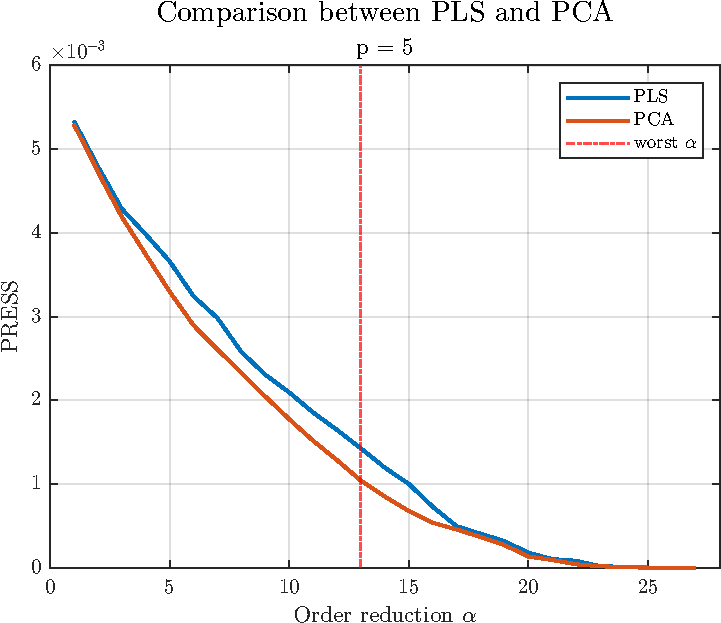
\includegraphics[width=\textwidth]{Images/PLS_vs_PCA.pdf}
		\end{subfigure}
	\end{figure}
	For the central orders PCA is slightly more accurate than PLS in the reconstruction of the matrix $X$ starting from the reduced domain. For the extreme orders, instead, the two techniques are similar.
\end{frame}

\begin{frame}
	\frametitle{Bibliography}
	\begin{block}{Book}
		\textbf{Fault Detection and Diagnosis in Industrial Systems}\\
		L. H. Chiang, E. L. Russel and R. D. Braatz
	\end{block}
		\begin{alertblock}{Dataset}
		\textbf{Faulty Steel Plates}\\
		\small{\url{https://www.kaggle.com/datasets/uciml/faulty-steel-plates}}
	\end{alertblock}
	\begin{exampleblock}{Repository GitHub}
		\small{\url{https://github.com/LorenzoF6/PLS_Algorithm_Implementation.git}}
	\end{exampleblock}
\end{frame}